\chapter{Terminierung des intrinsischen Delaunay-Refinement}
\label{kap:Terminierung}

% Die Intuition des Beweises zur Terminierung beruht auf zwei Faktoren. Zum einen ist die Fläche der Triangulierung begrenzt, kann somit nicht erweitert werden. Zum anderen ist gewährleistet, dass alle Kanten, die durch den Algorithmus hinzugefügt werden, eine minimale Länge haben. Das liegt daran, dass beim Einfügen von Knoten garantiert ist,  dass keine zwei Knoten zu nahe beieinander liegen können.
% Da folglich die Kanten nicht unendlich klein werden können und die Fläche nicht größer wird, können irgendwann keine neuen Kanten mehr erzeugt werden und der Algorithmus terminiert. \\




Im Folgenden werden wir zeigen, dass der Algorithmus für eine Eingabe garantiert terminiert, für die alle Knoten $i$ einen Gesamtwinkel $\gesamtwinkel*\geq \frac{\pi}{3}$ haben und einen Winkel-Schwellenwert $\kleinsterWinkel* \leq \frac{\pi}{6}$. In der Ausgabe des Algorithmus soll für alle Innenwinkel der Triangulierung gelten, dass sie größer gleich dem gegebenen Winkel-Schwellenwert $\kleinsterWinkel*$ sind. Erst, wenn diese Bedingungen erreicht ist, terminiert der Algorithmus.


% Aus dem Kreiswinkelsatz (\ref{fig:kreiswinkelsatz}) wissen wir, dass für den kleinsten Winkel $\alpha$ eines Dreiecks 
% \begin{align*}
%     \sin(\alpha) = \frac{d}{2\cdot r}  
% \end{align*}

% gilt.

% Wird hier für  $\alpha$ die Winkeluntergrenze \kleinsterWinkel eingesetzt erhalten wir die  Obergrenze $B$ des Ur-z-kK-Verhältnisses $B = \frac{\kuezesteKante*}{2 \umkreisradius*}$.
% %TODO Satz verbessern
% Daher ist die Winkeluntergrenze \kleinsterWinkel äquivalent zu einer Obergrenze $B$ des Ur-z-kK-Verhältnisses  $\frac{\kuezesteKante*}{2 \umkreisradius*}$.\\



%Kante $d_{min}$ der Eingabe sind
% Im Folgenden zeigen wir, dass der Algorithmus \algorithmusname keine Kanten erzeugen kann, die kürzer als ein von der Eingabe Triangulierung, abhängiges Minimum $E_{min}$ ist.  Der Algorithmus kann also nur maximal so lange neue Knoten einfügen, bis alle Knoten $E_{min}$ von ihren Nachbarn entfernt sind.


Da der Beweis mit  Längenrelationen arbeitet, führen wir Hilfsfunktionen ein, um Entfernungen besser zu beschreiben. 

\subsubsection{Hilfsfunktionen}
Die Hilfsfunktionen definieren verschiedene Längen, um später im Beweis mit ihnen arbeiten zu können.
\begin{definition}
Sei $M = (V,E,T)$ eine Delaunay-Triangulierung  einer geschlossenen StF-Oberfläche, sei $t \in T$ ein Dreieck aus $M$, sei $v,u \in V$ ein Knoten aus $M$ und sei $e_{(v,u)} \in V$ eine Kante aus $M$,  dann entspricht
\begin{itemize}
    \item $d(t)$ die Länge der kürzesten Seite von $t$
    \item $d(v)$ die Länge der kürzesten zu $v$ inzidenten Kante
    \item $d(v,u)$ die Länge der Kante  $e_{(v,u)}$
    \item $r(t)$ die Länge des Umkreisradius von $t$
    \item $N(v)$ einer Liste aller zu $v$ inzident Kanten
\end{itemize}


\end{definition}



Das folgende Lemma besagt, dass für einen Iterationsschritt die jeweils neu erzeugten Kanten adjazent zum neu eingefügten Knoten sind.


%   dass für eine Kante $e$ aus der neuen Triangulierung $M^\prime$, die nicht mit dem hinzugefügten Knoten $v$ verbunden ist, bereits in der alten Triangulierung $M$ enthalten sein muss.

\begin{figure}[h!]
    \centering
    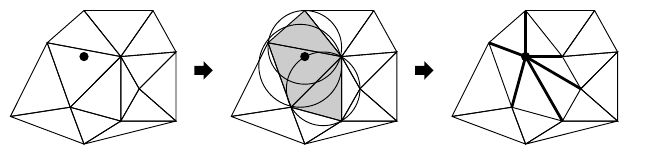
\includegraphics[width=5in]{images/adejazent.png}
    \caption{Illustration, dass alle neu erzeugten Kanten adjazent zum neu eingefügten Knoten sind \cite{shewchuk:1997:delaunay} }%\cite{shewchuk:1997:delaunay}}
    \label{fig:Punkt_einfügen}
\end{figure}
 


\begin{lemma}
\label{le:adejazent}
Sei $M = (V,E,T)$ eine intrinsische Delaunay-Triangulierung  einer geschlossenen  StF-Oberfläche und sei $M^\prime = (V^\prime,E^\prime,T^\prime)$ die Delaunay-Triangulierung  $M$ nach dem Einfügen eines neuen Knotens $v$.
 

%für jeden neu hinzugefügten Kante aus $M^\prime$, dass Sie adjazent zu $v$ ist.

%Beweis per Kontraposition: 
Wenn eine Kante $e \in E^\prime$ und $e \in N(v)$ ist und $e \in  N(v)$
%nicht Adjazent zu $v$ ,
dann folgt $e \not \in   E $.\\


% \begin{align*}
%     E^\prime \setminus E \equiv  N(v)\\
% \end{align*}


\end{lemma}

%Zeige: Ist eine Kante in der neuen Delaunay Triangulierung nicht mit dem neuen Knoten verbunden, so war sie schon in der alten Delaunay Triangulierung.


% \begin{definition}
% Eine Kante wird als Delaunay-Kante bezeichnet, wenn innerhalb der Kreisscheibe, die durch die beiden Entknoten verlauft, keine weiteren Knoten liegen.  
% \end{definition}



%Beweis per Kontraposition: wenn eine Kante $e \in E^\prime$ nicht adjazent zu $v$ ist, dann wahr sie auch in  $E$ enthalten. \\

%Angenommen es existiert in $M^\prime $ eine Kante $e \in E^\prime $  die nicht adjazent zu $v$ ist und für die gilt $e \not \in E $ 

\begin{proof}

%Beweis per Kontraposition: 
Angenommen $e \not \in  N(v)$, dann ist zu zeigen, dass $e\in E $ gilt.\\

Nach \cite[Definition 3]{Bobenko:2007:LaplaceBeltrami} ist eine Kante in einer Delaunay-Triangulierung  enthalten genau dann, wenn eine leere Kreisscheibe existiert, auf deren Rand nur ihre beiden Endknoten liegen.\\ 

    Wegen $V \subset V^\prime$  ist jede leere Kreisscheibe in $M^\prime$  auch in  $M$ enthalten. Per Annahme enthält $M$ auch beide Endknoten von $e$. Somit enthält $M$ auch $e$.     
\end{proof}


%und mindestens so lang wie ein von der Eingabe Triangulierung, abhängiges Minimum $E_{min}$ sind. 
Dünne Dreiecke sind Dreiecke mit mindestens einem Innenwinkel $\leq \frac{\pi}{6}$.  
Das nächste Lemma zeigt, dass für ein dünnes Dreieck der Umkreisradius mindestens so lang ist wie seine kürzeste Kante.


%  \citeauthor{chew:1989:guaranteed} zeigt bereits in  \cite{chew:1989:guaranteed,chew:1993:guaranteed}
%   für $\theta_{min} \leq 30^\circ$, dass sein Algorithmus terminiert.\\
%   das nächste Lemma zeigt, dass für ein als schlecht klassifizierten Dreiecke $t$ mit mindestens einem Innenwinkel kleiner $\theta_{min}$ ein  Ur-z-kK Verhältnisses größer gleich $1$ hat, in dem gilt, dass $ d(t) \leq r(t) $. 
   
% \begin{definition}
% Sei $B \geq 1 $ die Obergrenze des Ur-z-kK-Verhältnisses, so gilt jedes Dreieck mit einem Ur-z-kK Verhältnis größer $B$ als schlecht Dreieck.
% \end{definition}



% Sei B die Obergrenze dieser Metrik so gilt jedes Dreick mit einem Ur-z-kK Verhältnis grö-
% ßer als B als schlecht Dreieck. Delanuny Refinement Algorithmen könne diesen Wert nur
% verbessern und terminieren, wenn Sie für jedes Dreieck ein Wert kleiner B erzielt haben.

\begin{lemma}
\label{le:dünnes_dreieck}
Sei $t$ ein Dreieck mit kleinstem Winkel $\alpha \leq \frac{\pi}{6}$.\\
Dann gilt: 
 
 \begin{align*}
     r(t) \geq d(t).
 \end{align*} 
 \end{lemma}

\begin{figure}[h]
    \centering
    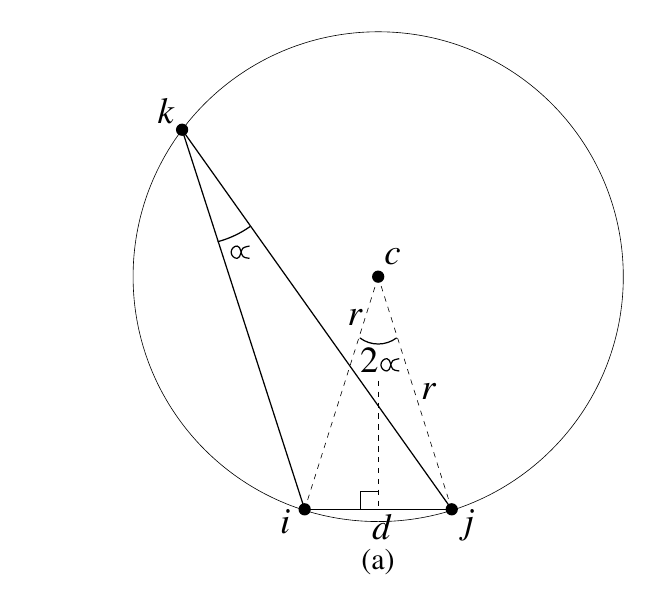
\includegraphics[width=3in]{images/Kreiswinkelsatz.png}
    \caption{Illustration des Kreiswinkelsatzes \cite{shewchuk:1997:delaunay}}
    \label{fig:kreiswinkelsatz}
\end{figure}


\newpage
\begin{proof}
Mithilfe des Kreiswinkelsatzes (\ref{fig:kreiswinkelsatz}) gilt:
\begin{align*}
d(t) &= r(t)\cdot 2\cdot\sin(\alpha)  \\
\end{align*}
Aus der Annahme $\alpha \in [0,\frac{\pi}{6}] $ folgt:

\begin{align*}
    \sin(\alpha) \leq \frac{1}{2}.
\end{align*}

Einsetzen in obige Gleichung ergibt 

\begin{align*}
     d(t) &\leq r(t).\\
\end{align*}
\end{proof}

Das nächste Lemma zeigt, dass der größte mögliche Umkreisradius bereits in der Eingabe-Triangulierung enthalten ist und durch das Einfügen neuer Punkte nur leere Kreisscheiben erzeugt werden, deren Radius kleiner gleich dem größten Radius der Eingabe ist. 



Aufgrund der Delaunay-Eigenschaft gilt jedoch, dass in der Kreisscheibe (also nicht außerhalb und nicht auf dem Rand) keine Kugelpunkte liegen. Infolgedessen ist für eingebettete leere Kreisscheiben garantiert, dass alle beteiligten Flächen sich gemeinsam und eindeutig flach in der Ebene auffalten lassen. Somit können eingebettete leere Kreisscheiben, für sich genommen, wie in der Ebene behandelt werden. 



\begin{lemma}
\label{le:auffaltung}
Sei $M = (V,E,T)$ eine intrinsische Delaunay-Triangulierung  einer geschlossenen StF-Oberfläche. Sei $K$  die größte leere Kreisscheibe auf $M$ und sei $M^\prime = (V^\prime,E^\prime,T^\prime)$ die Delaunay-Triangulierung  $M$ nach dem Einfügen eines neuen Knotens $v$. 
Dann gilt für die größte leere Kreisscheibe $K^\prime$ in $M^\prime$,

%_{i_{max},j_{max},k_{max}} mit $i_{max},j_{max},k_{max} \in V$,
\begin{align*}
    r(K) \geq r(K^\prime).\\
\end{align*}
\end{lemma}

\begin{proof}

Angenommen, durch das Einfügen von $v$ in $M$ entsteht eine neue leere Kreisscheibe $K^\prime$ mit 

\begin{align*}
    r(K^\prime) > r(K).
\end{align*}

Aus $V = V^\prime \setminus \{v\}$ und $K^\prime = \emph{}$ folgt $K^\prime \subset M$, da sie dann immer noch leer ist.\\ Das widerspricht der Annahme, dass $K$ die größte leere Kreisscheibe in $M$ ist.

\end{proof}


%  das Lemma \ref{le:dünnes_dreieck} zeigt, dass für ein $B  \geq 1$ der einfüge Radius durch eine Folge von Nachfahren eines
% Knotens nicht abnehmen Kannen. Wenn Knoten mit kleineren einfügeradien nicht erzeugt
% werden können, können keine Kanten eingeführt werden, die kürzer als die vorhandenen
% kanten sind, und die Delaunay-Verfeinerung terminiert garantiert.
% Bei der Triangulierung stückchenweise flachen-Oberfläche gibt es ein zusätzliches topologi-
% sches Besonderheit zu beachten, da sie Irregularität erlaubt, kann ein Knoten v eine Kante e
% zu sich selbst haben.




Bei Triangulierung von geschlossenen StF-Oberfläche gibt es im Vergleich zu Triangulierungen in der euklidischen Ebene zusätzliche topologische Besonderheiten zu beachten. Da sie irreguläre Dreiecke zulassen, kann ein Knoten $v$ eine Kante \irregulaereKante zu sich selbst haben.    



Die minimale Länge von regulären Kanten wird dadurch festgelegt, dass Knoten nicht zu nahe bei einander eingefügt werden können. Dies gilt nicht für irreguläre Kanten.
Dabei ist es wichtig zu unterscheiden, ob sie sich um ein Loch, einen Bereich mit kurzem Umfang oder Kegelspitze wickelt. Bei einem Loch oder einem Bereich mit kurzem Umfang existiert ebenfalls ein festes Minimum, nämlich der minimale Umfang der StF-Oberfläche. Diese lässt sich berechnen \cite{erickson:2005:generator}. Bei Kegelspitzen kann sich die Schleife  theoretisch unendlich klein zusammen ziehen. Daher müssen wir diesen fall gesondert betrachten.   



% Wir betrachten die in \cite [definition 3] {Bobenko:2007:LaplaceBeltrami}  eingeführte Definition zur Verallgemeinerung der Delauny-Triangulierung passen dabei  aber  Notation aber im Sinne der Konsistenz dieser Arbeit an.

% \begin{definition}
% Sei $M = (V,E,T)$ eine intrinsische Delaunay-Triangulation einer geschlossenen StF-Oberfläche.
% Die Delaunay-Zerlegung von $M$  ist die Vereinigung disjunkter Einheiten.
% die Delaunay-Zerlegung besteht dabei aus folgenden Mengen: Eine Teilmenge $ C \subset M$ ist eine geschlossene Einheit der Delaunay-Zerlegung, genau dann, wenn eine eingebettet leere Kreisscheibe existiert und auf ihrem Rand genau die Knoten aus $C$ liegen und zwar nur diese.
% dabei unterscheide man die Einheiten an der Anzahl ihrer Knoten: 1-Einheiten (Knoten), 2-Einheiten (Kanten) und 3-Einheiten (Dreiecksflächen)   
% \end{definition}

% Die gültige dieser Definition wurde in  \cite [Proposition 4 ff.] {Bobenko:2007:LaplaceBeltrami} gezeigt, würde an dieser Stelle aber den Rahmen dieser Arbeit sprengen.

% Es folgt unmittelbar aus der Definition: dass eine zugehöre Kante existiert, falls es eine eingebettete leere Kreisscheibe existiert, sodass die Endpunkte der Kante, und nur diese Punkte, auf dem Rand dieser Kreisscheibe liegen. Besagte Kante wird auch als Delaunay-Kante bezeichnet.



Da die Eingabetriangulierung im Allgemeinen regulär ist, können irreguläre Dreiecke erst durch das Wiederherstellen der Delaunay-Eigenschaft entstehen\cite{Bobenko:2006:SIGGRAPH,Bobenko:2007:LaplaceBeltrami}. Wir betrachten den Fall einer Schleife um eine Kegelspitze und zeigen, dass die erzeugte irreguläre Kante größer gleich der regulären Kante ist.


% nach dem Einfügen des Umkreismittelpunkts $v$ eines dünnen Dreiecks $t_{bad}$ in die Nachbarschaft einer sphärischen Kegelspitze $s$ entstehen.  
% Nun wollen wir zeigen, wann die erzeugte irreguläre Kante  \irregulaereKante von $v$ nach $v$  größer gleich der regulären Kante \regulaereKante ist.

% \begin{align*}
%     \regulaereKante* &\leq \irregulaereKante*\\
% \end{align*}


 \begin{figure}[h]
    \centering
    


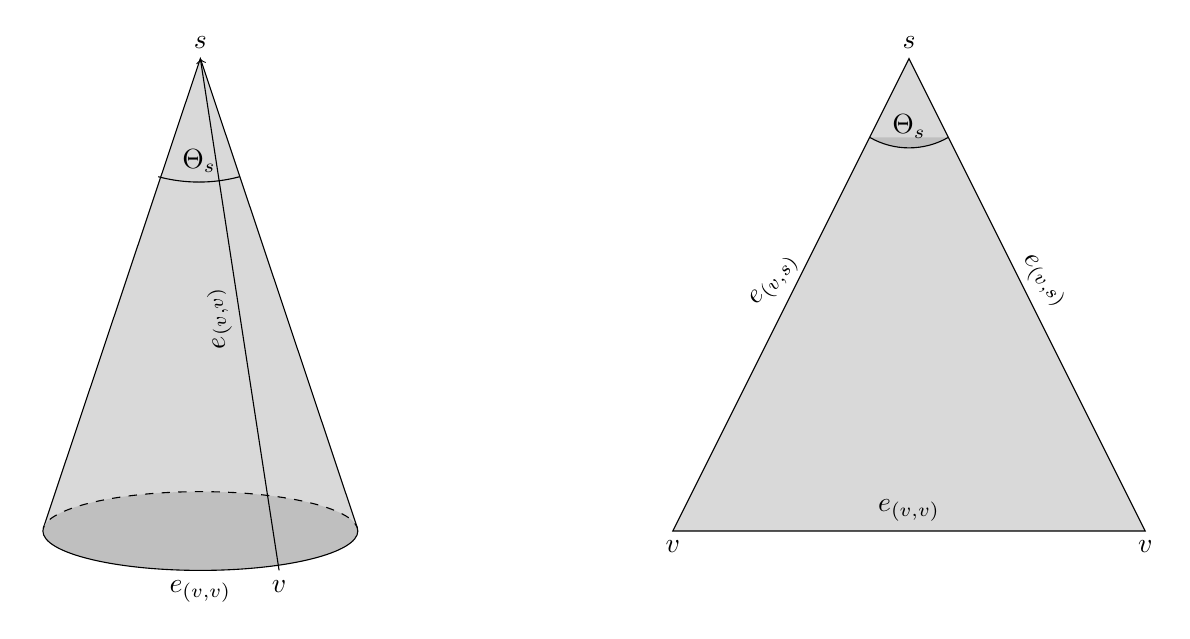
\begin{tikzpicture}

\usetikzlibrary{calc}
\newcommand{\radiusx}{2}
\newcommand{\radiusy}{.5}
\newcommand{\height}{6}

  \newcommand{\delayx}{6}

\coordinate (a) at (-{\radiusx*sqrt(1-(\radiusy/\height)*(\radiusy/\height))},{\radiusy*(\radiusy/\height)});

\coordinate (b) at ({\radiusx*sqrt(1-(\radiusy/\height)*(\radiusy/\height))},{\radiusy*(\radiusy/\height)});





\draw[fill=gray!30] (a)--(0,\height)--(b)--cycle;

\fill[gray!50] circle (\radiusx{} and \radiusy);

\begin{scope}
\clip ([xshift=-2mm]a) rectangle ($(b)+(1mm,-2*\radiusy)$);
\draw circle (\radiusx{} and \radiusy);
\end{scope}

\begin{scope}
\clip ([xshift=-2mm]a) rectangle ($(b)+(1mm,2*\radiusy)$);
\draw[dashed] circle (\radiusx{} and \radiusy);
\end{scope}

%\draw[dashed] (0,\height)|-(\radiusx,0) node[right, pos=.25]{$h$} node[above,pos=.75]{$r$};
%\draw (0,.15)-|(.15,0);


\draw  ( 0,\height) coordinate (a)  (\radiusx,0) coordinate (b) (-1* \radiusx ,0) coordinate (c); 

% \pic[draw=orange,<->,angle radius=\radiusx * 20,fill=teal!30]{angle=c--a--b};
\draw  (0+0.5,\height-1.5) arc (-75:-105:2) node[above,midway]{$\Theta_{s}$};


\draw[->](\radiusx/2,-\radiusy)--node[above,rotate=100] {$e_{(v,v)}$} (0,\height);
\coordinate[label=below:$v$] (d)  at (\radiusx/2,-\radiusy);
\coordinate[label=below:$e_{(v,v)}$] (d)  at (0,-\radiusy);
\coordinate[label=above:$s$] (c) at (0,\height);


\draw[fill=gray!30]   (0+\delayx,0) coordinate[label=below:$v$] (a) -- node[above,rotate=50] {$e_{(v,s)}$} 
        (3+\delayx,6) coordinate[label=above:$s$] (b) -- node[above,rotate=-50] {$e_{(v,s)}$}
        (6+\delayx,0) coordinate[label=below:$v$] (c) --node[above] {$e_{(v,v)}$}  cycle;
        
    \draw[fill=gray!50]  ({3+\delayx+.5},{6-1}) arc (-60:-120:1) node[above,midway]{$\Theta_{s}$};
    




\end{tikzpicture}


    \caption{Illustration der Auffaltung eines irregulären Dreiecks in der euklidischen Ebene  }%\cite{shewchuk:1997:delaunay}}
    \label{fig.irreglaere}
\end{figure}

\begin{lemma}
\label{le:irregulär_entfernung}
Sei $M = (V,E,T)$ eine intrinsische Delaunay-Triangulierung  einer geschlossenen  StF-Oberfläche und  $t \in T$ ein irreguläres Dreieck aus $M$. 

%Sei $v \in t$ der zuletzt eingefügt Knoten im Dreieck $t$  und $s \in t$ eine sphärische Kegelspitze mit einem Gesamtwinkel $\gesamtwinkel*[s] \in [0,180^\circ] $. Weiterhin beschreibt \irregulaereKante die irreguläre Kante $(v,v)\in E$.\\  

Seien $v,s \in V$ die Knoten von t, \irregulaereKante die irreguläre Kante und Kegelwinkel \gesamtwinkel[s] von s gilt $\gesamtwinkel*[s] \in [\frac{\pi}{3}, \pi]$

%Wenn für alle  $v \in V$:  $\gesamtwinkel*[v] \geq 60^\circ$ gilt,
Dann folgt:
%wenn  alle Kegelspitzen in $M$ mit einem Gesamtwinkel, $\gesamtwinkel* \leq 60^\circ $ besitzt, dann gilt 
\begin{align*}
    d(\irregulaereKante*) \geq d(\regulaereKante*).\\
\end{align*}  

\end{lemma}

\begin{proof}

% laut \ref{le:regulär_entfernung} wissen wir
% Nehmen wir an, dass die regulären Kanten $e_{(s,v)}$ und $e_{(v,s)}$ zwischen $s$ und $v$ sind, größer gleich  $r_{t}$.


Aus dem Kosinussatz folgt 
\begin{align*}
    d(\irregulaereKante*^2) &=  d(e_{(s,v)})^2 + d(e_{(v,s)})^2-2 \cdot d(e_{(s,v)})  \cdot d(e_{(v,s)}) \cdot \cos(\gesamtwinkel*[s]). \\
\end{align*}

Da $d(e_{(s,v)}) = d(e_{(v,s)})$ gilt, erhalten wir durch Umformung

\begin{align*}
    % d(\irregulaereKante*)^2 &=   2\cdot d(\regulaereKante*)^2 - 2\cdot d(\regulaereKante*)^2 \cdot \cos(\gesamtwinkel*[s]) \Leftrightarrow\\ 
    % \d(\irregulaereKante*)^2 &= 2\cdot d(\regulaereKante*)^2 \cdot (1- \cos(\gesamtwinkel*[s]))\Leftrightarrow\\
    d(\irregulaereKante*)&= \sqrt{2 (1-\cos(\gesamtwinkel*[s]))}\cdot d(\regulaereKante*).\\
\end{align*}

% Nun setzten wir $\sqrt{2 (1-\cos(\gesamtwinkel*))}\cdot d(\regulaereKante*)$ für  $d(\irregulaereKante$ ein 
% \begin{align*}
%  \sqrt{2 (1-\cos(\gesamtwinkel*))}\cdot d(\regulaereKante*) \geq d(\regulaereKante*).\\   
% \end{align*}
wegen $\gesamtwinkel*[s] \in  [\frac{\pi}{3}, \pi]$, also $-1 \leq \cos(\gesamtwinkel*[s]) \leq \frac{1}{2}$  folgt
%Damit die Abschätzung gilt, muss 

\begin{align*}
     \sqrt{2 (1-\cos(\gesamtwinkel*[s]))} \geq \sqrt{2 (1-\frac{1}{2})} \geq 1\\
\end{align*}

und damit $\irregulaereKante* \geq \regulaereKante* $. 


\end{proof}


%  Lemma \ref{le:irregulär_entfernung} zeigt also, dass \algorithmusname nur irreguläre Triangulationen erzeugt, in denen die irregulären Kanten mindestens so lang sind wie die regulären Kanten des Dreiecks.\\  

Das folgende Lemma zeigt, dass durch den Algorithmus erzeugte reguläre Kanten nicht kleiner als der entsprechende Umkreisradius $r(t_{bad})$ des dünnen Dreiecks $t_{bad}$ sein können, aus dem sie erzeugt wurden.

\newpage
\begin{lemma}
\label{le:regulär_entfernung}
Sei $M = (V,E,T)$ eine Delaunay-Triangulierung  einer geschlossenen StF-Oberfläche, sei $t \in T$ ein Dreieck aus $M$, sei $v$ der Umkreismittelpunkt von $t$.   \\

 

%für alle Knoten $u\in V$ das sie mindestens $r_t$ von v entfernt sind. 


Nach dem Einfügen von $v$ in $M$ und der Wiederherstellung der Delaunay-Eigenschaft gilt für jede neu erzeugte reguläre Kante $e$, dass sie adjazent zu $v$ ist, und dass 
\begin{align*}
    d(e) \geq r(t) 
\end{align*} gilt.
%$\forall e.e\in N(v) $
\end{lemma}
 \begin{figure}[h]
    \centering
    \includegraphics[width=3in]{images/regulär_entfernung.png}
    \caption{Illustration, dass durch die Delaunay-Eigenschaft gewährleistet wird, dass neu eingefügte Knoten nicht zu nahe an bestehen Knoten liegen    \cite{SHEWCHUK:2002:chuws}}
    \label{fig:regulär_entfernung}
\end{figure}

\begin{proof}
Da $M$ die Delaunay-Eigenschaft besitzt, gilt für alle Dreiecke $t\in T$ die Delaunay-Eigenschaft, die besagt, dass im Umkreis von $t$ keine Knoten liegen, die nicht zu $t$ gehören. Nach dem Einfügen von $v$ in $M$ und dem Wiederherstellen der Delaunay-Eigenschaft gilt also für alle neu hinzugefügten regulären Kanten, dass sie inzident zu $v$ (\ref{le:adejazent}) und somit mindestens $r(t)$ lang sind.
\end{proof}

% \begin{remark}
% Eine Triangulation wird als regulär bezeichnet, wenn jedes Dreieck aus drei  Kanten und drei Knoten besteht, die jeweils paarweise verschieden sind.
% \end{remark}

% \begin{remark}
% Ein Dreieck gilt als schlecht, wenn es mindestens einen Innenwinkel $\innenwinkel* \leq 30^\circ $ besitzt.
% \end{remark} 
\newpage
Der folgende Beweis vereint nun die in den Lemmata aufgestellten Längenrelationen und zeigt, dass der Algorithmus nur Kanten erzeugen kann, die eine durch die Eingabe bestimmte Mindestlänge haben.

\begin{lemma}
\label{lem:Obergrenze}
Sei $M = (V,E,T)$ eine Delaunay-Triangulierung   einer geschlossenen StF-Oberfläche, sei $d_{min}$ die kürzeste Distanz zwischen zwei Knoten von $M$, sei $g_{min}$ der kürzeste Umfang von $M$ und sei $K_{max}$ die größte leere Kreisscheibe von $M$.

Angenommen, $M$ hat keine Kegelspitze $s$ mit einem Gesamtwinkel $\gesamtwinkel*[s] \leq \frac{\pi}{3}$. 

dann  existiert ein 
\begin{align*}
    \kappa^* = \frac{\min(d_{min}, g_{min} )}{r(K_{max)}}
\end{align*}
mit 
\begin{align*}
 \kappa^* \leq \kappa   
\end{align*}
für alle Dreiecke aus $M$.




\end{lemma}



\begin{proof}

Laut Lemma \ref{le:auffaltung} kann der Algorithmus keine Umkreisradien größer $r(k_{max})$ erzeugen.

Nehmen wir an, dass der Algorithmus \algorithmusname eine Kante, die kürzer als $\min(d_{min}, g_{min} )$ ist, einfügt. Sei \regulaereKante[(v,u)] die erste Kante dieser Art. Nach Lemma \ref{le:adejazent} ist \regulaereKante[(v,u)] inzident zum zuletzt eingefügten knoten. Sei dieser $v$ und $t_{bad}$ das zugehörige dünne Dreieck. \\

Da vor dem Einfügen von $v$ keine Kante kürzer als $\min(d_{min}, g_{min} )$ existiert hat, gilt  
\begin{align*}
    d(t_{bad}) \geq d_{min}.\\
\end{align*} 

Gemäß Lemma \ref{le:irregulär_entfernung} und \ref{le:regulär_entfernung} gilt, wenn \regulaereKante[(v,u)] eine reguläre Kante oder eine irreguläre Kante um eine Kegelspitze ist, die Abschätzung

\begin{align*}
    d(\regulaereKante*[(v,u)]) \geq r(t_{bad}).\\
\end{align*} 


Da $t_{bad}$ dünn ist, gilt nach Lemma \ref{le:dünnes_dreieck} 
\begin{align*}
    r(t_{bad}) \geq d(t_{bad}).
\end{align*}


 Daraus folgt  
 \begin{align*}
     d(\regulaereKante*[(v,u)]) \geq d_{min}.
 \end{align*}

Weiterhin gilt, wenn \regulaereKante[(v,u)] eine Schleife um einen Bereich mit kurzem Umfang oder ein Loch ist, nach Definition

\begin{align*}
     d(\regulaereKante*[(v,u)]) \geq g_{min}.
 \end{align*}



Das steht jedoch im Widerspruch zu der Annahme, dass \regulaereKante[(v,u)] kürzer ist als $\min(d_{min}, g_{min} )$. Es folgt also, dass keine eingefügte Kante kürzer ist als $\min(d_{min}, g_{min} )$. Somit kann der Algorithmus keine Dreiecke erzeugen mit \\
 \begin{align*}
    \kappa^* = \frac{ \min(d_{min}, g_{min} )}{r(k_{max})} \leq \kappa.
 \end{align*}

\end{proof}

In Lemma \ref{lem:Obergrenze} haben wir gezeigt, dass der Algorithmus nur Dreiecke erzeugt mit $\kappa \geq \kappa* $.

Nun wollen wir zeigen, dass \algorithmusname aufgrund der begrenzten Fläche terminiert. Da die Fläche der Eingabetriangulierung endlich ist, der Algorithmus in jeder Iteration neue Dreiecke erzeugt und diese Dreiecke wiederum eine Mindestfläche $A_{min}$ haben, folgt, dass der Algorithmus terminieren muss, sobald er die zur Verfügung stehende Gesamtfläche nicht mehr weiter aufteilen kann.\\  



\begin{theorem}
Sei $M = (V,E,T)$ eine Triangulierung einer geschlossenen StF-Oberfläche.
Angenommen, $M$ hat keine Kegelspitze $s$ mit einem Gesamtwinkel $\gesamtwinkel*[s] \leq \frac{\pi}{3}$ und sei  $\kleinsterWinkel* \leq \frac{\pi}{6}$ ein Winkel-Schwellenwert. 


Das intrinsische Delaunay-Refinement mit $M$ und \kleinsterWinkel als Eingabe terminiert.
\end{theorem}


% \begin{proof}
% Sei $t$ ein Dreieck aus $M$ mit einem Verhältnis von Umkreisradius zu kürzester Kante \UrzkK, Flächeninhalt $A$ und kleinsten Winkel $\theta_{min}$.




% Laut Kreiswinkelsatz gilt 
% \begin{align*}
% \theta_{min} = \arcsin(\frac{\UrzkK*}{2}) 
% \end{align*}

% Aus dem Sinussatz folgt 
% \begin{align*}
%     A \geq \frac{1}{2} \sin(\theta_{min}) \cdot d(t)^2
% \end{align*}

% Nach Lemma \ref{lem:Obergrenze} ist 
% \begin{align*}
%     \kappa \geq \kappa^* 
% \end{align*}

% Daraus folgt, dass auch eine untere Grenze für $A$ existiert und somit jedes neu erzeugte Dreieck eine Mindestfläche hat.
% \end{proof}

\begin{proof}
das lemma \ref{lem:Obergrenze} zeigt, dass es keine Kante kürzer ist als  \begin{align*}
    D = \min(d_{min},g_{min})
\end{align*}

und eine Untergrenze \begin{align*}
    \kappa^* \leq \frac{\min(d_{min},g_{min})}{r(k_{max})}
\end{align*}

von $\kappa$ existiert.

Aus dem Kreiswinkelsatz folgt, es existiert ebenfalls eine Winkeluntergrenze 

\begin{align*}
    A = \sin(\frac{\kappa^*}{2})
\end{align*}
für jedes Dreieck.\\
Aus dem Sinussatz folgt, dass jedes Dreieck eine Mindestfläche von \begin{align*}
    \frac{1}{2} \cdot \sin(A)D^2 
\end{align*}
hat.\\

Insgesamt ist die Fläche der Eingabetriangulierung begrenzt und jedes Dreieck hat eine Mindestfläche. Der Algorithmus erzeugt in jedem Schritt neue Dreiecke und da der Algorithmus nur Dreiecke mit endlich kleine Flächen erzeugen kann, muss er schließlich terminieren
\end{proof}








